\documentclass[letterpaper,12pt]{article}
\usepackage[margin=1in]{geometry} 
\usepackage[bottom]{footmisc}
\usepackage{amsmath}
\usepackage{tcolorbox}
\usepackage{amssymb}
\usepackage{amsthm}
\usepackage{lastpage}
\usepackage{fancyhdr}
\usepackage{accents}
\usepackage{mathtools}
\usepackage[numbered,framed]{matlab-prettifier}
\usepackage{listings}

\pagestyle{fancy}
\setlength{\headheight}{40pt}


\newenvironment{solution}
  {\renewcommand\qedsymbol{$\blacksquare$}
  \begin{proof}[Solution]}
  {\end{proof}}
\renewcommand\qedsymbol{$\blacksquare$}

\newcommand{\ubar}[1]{\underaccent{\bar}{#1}}
\newcommand{\nlim}[1]{{\lim_{n \rightarrow \infty}{#1}}} % add packages, settings, and declarations in settings.tex

\begin{document}

\lhead{Jonathan Thompson} 
\rhead{MATH 5470 Fall 2022 \\ Laplace's Equation - Circular Annulus Plots} 
\cfoot{}

For Problem 1(a), our solution is given by:

$$
u(r, \theta) = \frac{4 \ln{\frac{r}{5}}}{\ln{\frac{3}{5}}}
$$

We plot a (literal) heatmap and $u(r)$ below: 
\begin{figure*}[h]
    \centering
    \begin{subfigure}[b]{0.475\textwidth}
        \centering
        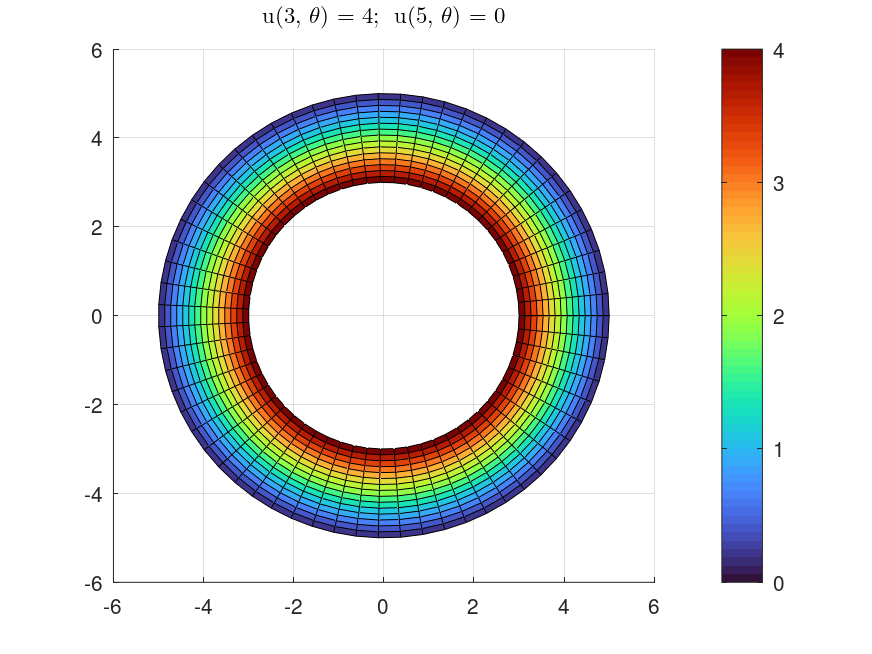
\includegraphics[width=\textwidth]{problem_1a_heatmap.png}
        \caption{Circular Annulus heatmap}
    \end{subfigure}
    \hfill
    \begin{subfigure}[b]{0.475\textwidth}
        \centering
        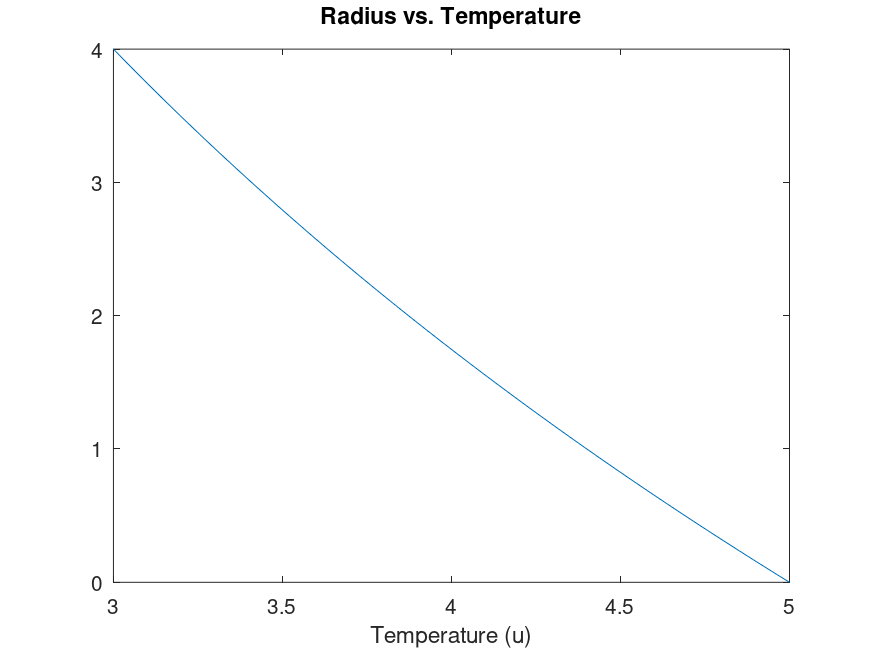
\includegraphics[width=\textwidth]{problem_1a_u_vs_r.png}
        \caption{$u$ vs. $r$}
    \end{subfigure}
    \caption[]{$u(r, \theta)$ for $u(3, \theta) = 4$ and $u(5, \theta) = 0$}
\end{figure*}

Similarly, for Problem 1(b), our solution is given by:

$$
u(r, \theta) = \frac{4 \ln{\frac{r}{3}}}{\ln{\frac{5}{3}}}
$$

with corresponding plots:

\begin{figure*}[h]
    \centering
    \begin{subfigure}[b]{0.475\textwidth}
        \centering
        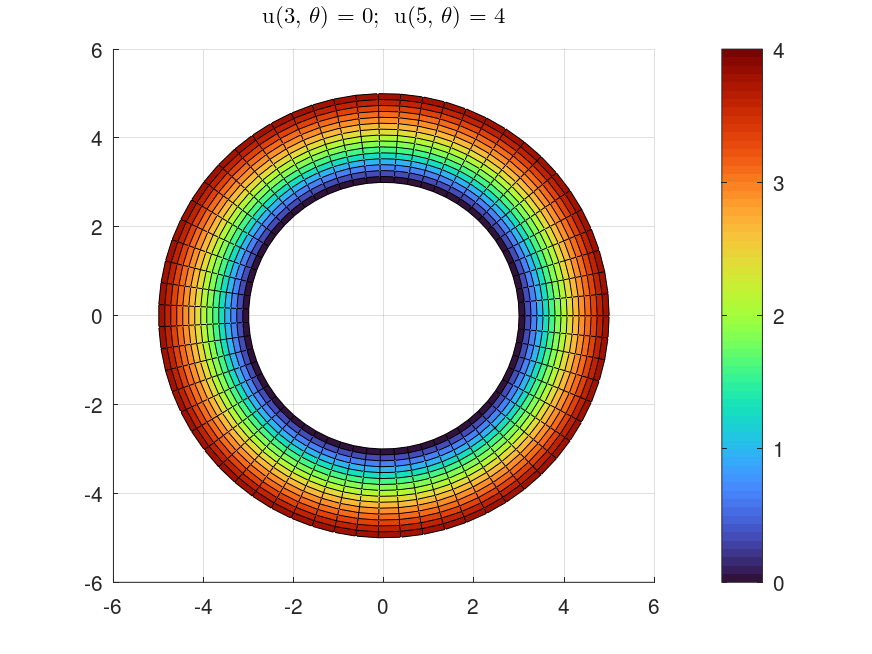
\includegraphics[width=\textwidth]{problem_1b_heatmap.png}
        \caption{Circular Annulus heatmap}
    \end{subfigure}
    \hfill
    \begin{subfigure}[b]{0.475\textwidth}
        \centering
        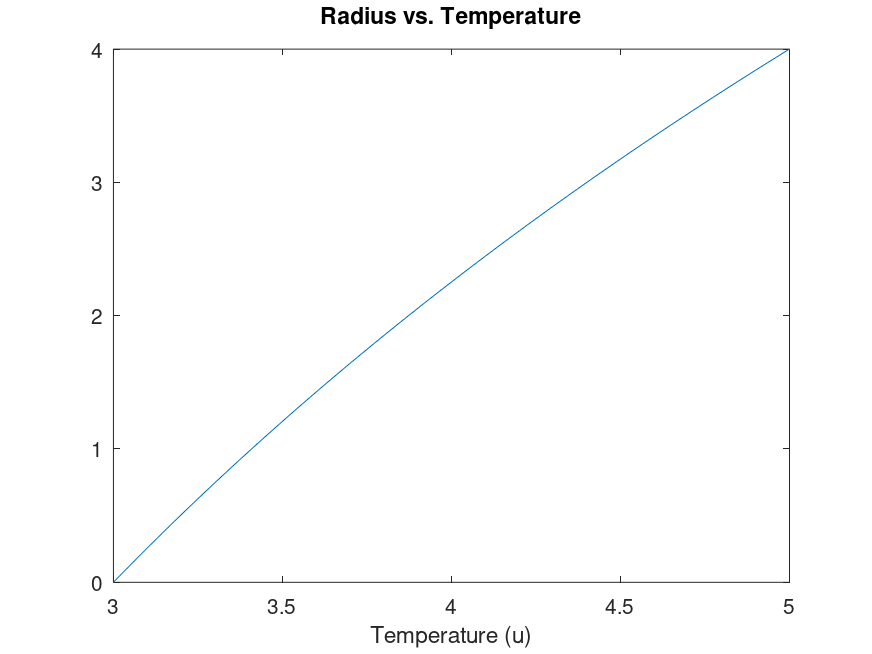
\includegraphics[width=\textwidth]{problem_1b_u_vs_r.png}
        \caption{$u$ vs. $r$}
    \end{subfigure}
    \caption[]{$u(r, \theta)$ for $u(3, \theta) = 0$ and $u(5, \theta) = 4$}
\end{figure*}

\end{document}
